% Compact PGFPlots panel for sampled surface7 BSC bit-scale decomposition.
% Requires \usepackage{pgfplots} and \pgfplotsset{compat=1.18}.
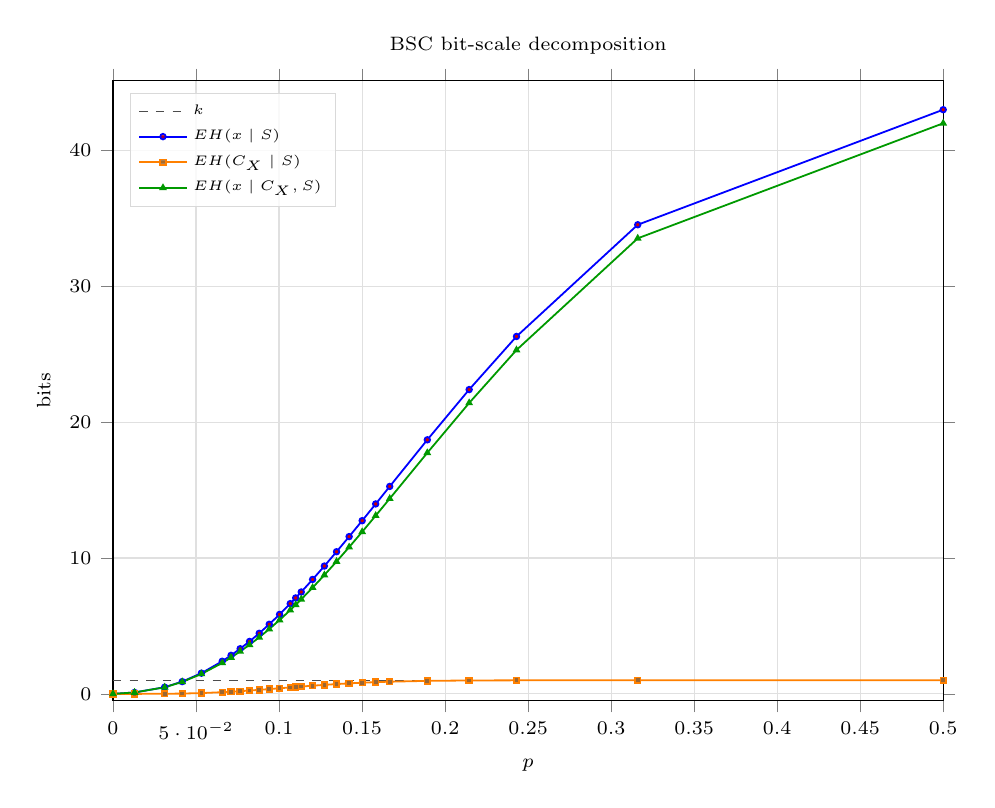
\begin{tikzpicture}
\begin{axis}[
  name=Surface7BSCBitScaleAxis,
  width=\linewidth,
  height=0.78\linewidth,
  title={BSC bit-scale decomposition},
  title style={font=\scriptsize},
  xlabel={$p$},
  ylabel={bits},
  xmin=0, xmax=0.5,
  ymin=-0.5, ymax=45.15,
  grid=both,
  major grid style={black!12},
  minor grid style={black!6},
  tick align=outside,
  tick label style={font=\scriptsize},
  label style={font=\scriptsize},
  legend cell align={left},
  legend style={draw=black!15, fill=white, fill opacity=0.82, text opacity=1, at={(0.02,0.98)}, anchor=north west, font=\tiny},
]
\addplot[black!70, dashed, line width=0.55pt] coordinates {(0,1) (0.5,1)};
\addlegendentry{$k$}
\addplot+[color=blue, mark=*, mark size=1.0pt, line width=0.65pt]
coordinates {(0,0) (0.0129868620555,0.103884980125) (0.0311244603048,0.491266352739) (0.0416926902737,0.902511710366) (0.0532390407768,1.52445506886) (0.0657867063546,2.40006093513) (0.0710958755299,2.83578004925) (0.0765765344037,3.32358680823) (0.0822333323659,3.85907062149) (0.0880715694979,4.45939182569) (0.0940972433461,5.12276147962) (0.100317108961,5.84887262429) (0.106738753821,6.64195821708) (0.110027864438,7.0637025978) (0.113370689941,7.49960369152) (0.120222466333,8.42169300242) (0.127304805976,9.41023509291) (0.134629772869,10.4619917578) (0.142210976498,11.5763953878) (0.150063823499,12.7481695242) (0.158205829694,13.9802654593) (0.166657010397,15.2681641725) (0.189297705371,18.7012302998) (0.21450174486,22.4000005308) (0.243003853809,26.3075558643) (0.316019346324,34.5316145176) (0.5,43)};
\addlegendentry{$\mathbb{E}H(x\mid S)$}
\addplot+[color=orange, mark=square*, mark size=1.0pt, line width=0.65pt]
coordinates {(0,0) (0.0129868620555,0.000214410560831) (0.0311244603048,0.0073089177615) (0.0416926902737,0.02333876461) (0.0532390407768,0.0584885061449) (0.0657867063546,0.123780731121) (0.0710958755299,0.159097463508) (0.0765765344037,0.199393495071) (0.0822333323659,0.245259590495) (0.0880715694979,0.296895434031) (0.0940972433461,0.352654612091) (0.100317108961,0.412936933871) (0.106738753821,0.476420276081) (0.110027864438,0.508128718257) (0.113370689941,0.539487400153) (0.120222466333,0.601468513875) (0.127304805976,0.663424330277) (0.134629772869,0.720338243567) (0.142210976498,0.774311924684) (0.150063823499,0.821414778638) (0.158205829694,0.862021967209) (0.166657010397,0.896675695721) (0.189297705371,0.957385963129) (0.21450174486,0.98654697695) (0.243003853809,0.996931511218) (0.316019346324,0.999986943301) (0.5,1)};
\addlegendentry{$\mathbb{E}H(C_X\mid S)$}
\addplot+[color=green!60!black, mark=triangle*, mark size=1.0pt, line width=0.65pt]
coordinates {(0,0) (0.0129868620555,0.103670569564) (0.0311244603048,0.483957434978) (0.0416926902737,0.879172945756) (0.0532390407768,1.46596656272) (0.0657867063546,2.27628020401) (0.0710958755299,2.67668258575) (0.0765765344037,3.12419331315) (0.0822333323659,3.61381103099) (0.0880715694979,4.16249639166) (0.0940972433461,4.77010686753) (0.100317108961,5.43593569042) (0.106738753821,6.165537941) (0.110027864438,6.55557387954) (0.113370689941,6.96011629137) (0.120222466333,7.82022448854) (0.127304805976,8.74681076264) (0.134629772869,9.7416535142) (0.142210976498,10.8020834631) (0.150063823499,11.9267547455) (0.158205829694,13.1182434921) (0.166657010397,14.3714884768) (0.189297705371,17.7438443367) (0.21450174486,21.4134535538) (0.243003853809,25.310624353) (0.316019346324,33.5316275743) (0.5,42)};
\addlegendentry{$\mathbb{E}H(x\mid C_X,S)$}
\end{axis}
\end{tikzpicture}
